%% Japanese manuscript for Memoirs of the Faculty of Engineering
% 工学部研究紀要日本語用TeXテンプレート
% ver. 2004.07.29
\documentclass[twocolumn,fleqn,10pt]{jarticle}
\usepackage[dvips]{graphicx}
\usepackage{overcite}%%superscript citation
\usepackage{times}%% use times font
% \usepackage{ulem}%%下線用
\usepackage{amsmath}
\usepackage{bm}
\usepackage{here}
\usepackage{nidanfloat}

%\usepackage{tabularx}%%expanded talbe environment
\renewcommand{\refname}{\normalsize 参考文献}

%% size definition (A4 = 210 mm * 297 mm)
\setlength{\oddsidemargin}{-1in}
\addtolength{\oddsidemargin}{20mm}
\setlength{\textwidth}{170mm}%210-20*2=170
%\setlength{\topmargin}{-1in}
\setlength{\topmargin}{-1.3in}
\setlength{\headsep}{0mm}
\setlength{\textheight}{253mm}%297-24-19=254
\setlength{\headheight}{24mm}
%\setlength{\footheight}{0mm}

\renewcommand\citeform[1]{[#1]}%%citation numcer with []
%\baselineskip=15pt %%baseline skip
%\renewcommand{\baselinestretch}{1.21}\tiny\normalsize%%baseline skip
\renewcommand{\baselinestretch}{1.03} %%baseline skip
\setlength{\columnsep}{12mm}%separation of column
\setlength{\mathindent}{8mm}%indent for equation
\footnotesep=10pt %line separation for footnote
%\parindent=1zw %indent at the beginning of the paragraph
\newfont{\titlefont}{cmbx10 scaled\magstep1}%%font for title (12pt computer modern bold)
\newfont{\authfont}{cmbx10 scaled\magstephalf}%%font for subtitle and authors (11pt computer modern bold)

%definition of abstract style
\makeatletter
\long\def\abstract#1{\def\@abstract{#1}}%
\def\@abstract{}
\long\def\jtitle#1{\def\@jtitle{#1}}%
\def\@jtitle{}
\long\def\jauthor#1{\def\@jauthor{#1}}%
\def\@jauthor{}
\let\@oldmaketitle\@maketitle%
\def\@maketitle{%
\centerline{
\begin{minipage}{140mm}
\begin{center}
 \vskip10mm
 \bfseries\@jtitle
 \vskip6mm
 \bfseries\@jauthor
\end{center}
\end{minipage}
}
 \vskip-1mm
 \@oldmaketitle
% \centerline{\bfseries\abstractname}%
 \leftmargini15mm
 \begin{quotation}\@abstract\end{quotation}%
 \vskip9mm}%
\makeatother

\makeatletter
\renewcommand{\section}{\@startsection
{section}{3}{0mm}{5mm}{5mm}{\bfseries \normalsize}}
\makeatother
\renewcommand{\thesection}{\arabic{section}.}

\makeatletter
\renewcommand{\subsection}{\@startsection
{subsection}{3}{0mm}{5mm}{0.01pt}{\bfseries \normalsize}}
\makeatother
\renewcommand{\thesubsection}{\arabic{section}.\arabic{subsection}}

\renewcommand{\thefootnote}{\fnsymbol{footnote}}%%footnote with marks

%%%%%%%%%%%%画像や表の「:」を消す処理%%%%%%%%%%%%%%
\makeatletter
\long\def\@makecaption#1#2{%
\vskip\abovecaptionskip
\iftdir\sbox\@tempboxa{#1\hskip1zw#2}%
\else\sbox\@tempboxa{#1\ #2}%
\fi
\ifdim \wd\@tempboxa >\hsize
\iftdir #1\hskip1zw#2\relax\par
\else #1\ #2\relax\par\fi
\else
\global \@minipagefalse
\hbox to\hsize{\hfil\box\@tempboxa\hfil}%
\fi
\vskip\belowcaptionskip}
\makeatother
%%%%%%%%%%%%%%%%%%ここまで%%%%%%%%%%%%%%%%%%%%%%%

%%日本語タイトル
\jtitle{%
{\Large
{\rm 電力使用量予測のための深層学習手法における\\最適なモデル選択に向けて}
}\\[3pt]
%{\large

%}
}

%%日本語著者
\jauthor{
%\scalebox{0.9167}{\large{\rm 増田 進也\footnotemark[1] 小高 知宏\footnotemark[2] 黒岩 丈介$^{\ast \ast \ast}$ 白井 治彦\footnotemark[1]}}
\scalebox{0.9167}{\large{\rm 山名田 恭吾* 黒岩 丈介** 
小高 知宏** 諏訪 いずみ*** 白井 治彦****}}
}

%English title
\title{%
\vspace{-4mm}
%\textbf{%
{\titlefont
An Investigation of Optimal Model Selection in Deep Learning Methods \\ for Electricity Usage Prediction
% \\\vspace{-4mm}Constant Monitoring of Traffic
}\\
%\vspace{-4mm}
%{\authfont
%-- Designing and implementation of DTI Hub --}
%\vspace{-1mm}
}


%Authors in English
\author{%
%\textbf{%
Kyogo YAMANADA*,{\hspace{3mm}}
Jousuke KUROIWA**,
Tomohiro ODAKA**\\
Izumi SUWA*** and
Haruhiko SHIRAI****
%{\authfont Shinya MASUDA}\protect\footnotemark[1],
%{\authfont Tomohiro ODAKA}\protect\footnotemark[2],
%{\authfont and}
%{\authfont Haruhiko SHIRAI}\protect\footnotemark[7],
%{\authfont Josuke KUROIWA}\protect $^{\ast \ast \ast}$,
%{\authfont and}
%{\authfont Hisakazu OGURA}\protect $^{\ast \ast \ast}$
%Please see the lines just after "\maketitle"
%}
\vspace{2mm}
}

%date
\date{
\normalsize (Received February 1, 2023)
\vspace{-3mm}
}

\abstract{



% 概要

In this paper, we investigate deep learning methods to predict electricity consumption. 
%Prediction of electricity consumption can be useful in the short term for setting the appropriate amount of electricity to be generated by power plants, and in the long term for appropriate procurement of fossil fuels required by each season. 
We employ RNN (Recurrent Neural Network) and LSTM (Long Short-Term Memory), both of which are applicable in handling time-series data, to predict electricity usage.
The target data are hourly, daily, and weekly electricity consumption data. 
%Mean square error of squared error (RMSE) is applied to evaluate the prediction results. 
The purpose of this paper is to investigate prediction accuracy for various structures of RNN and LSTM. 
The results show that the prediction accuracy surely depends on either RNN or LSTM and its structure for each of the hourly, daily, and weekly forecasts.



% 本研究では,深層学習を用いた電力使用量の予測を行った.
% 電力使用量の予測を行うことにより,短期的には発電所の発電量を適切に設定することができ,長期的には季節ごとに求められる化石燃料の適切な調達をすることに役立つ.
% 我々は,電力使用量の予測のために,時系列データを扱うことに長けている RNN(Recurrent Neural Network)と LSTM(Long Short-Term Memory)を用いて予測を行った.
% 対象データは時間ごと,日ごと,週ごとの電力使用量のデータとした.
% 予測結果の評価には平均平方二乗誤差(RMSE)を用いた.
% 結果として時間ごと,日ごと,週ごとのそれぞれの予測において適切な構造があることがわかった.





\vspace{1mm}
\begin{description}
\item[Key words :{\it Electric Usage Prediction, Deep Learning, RNN, LSTM}]
\end{description}
}
\vspace{-10mm}

\renewcommand*{\footnoterule}{\noindent\smash{\rule[3pt]{\linewidth}{0.4pt}}}

%%%%%%%%%%%%%%%%%%%%%%%%%%%%%%%%%%%%%%%%%%%%%%%%
\begin{document}

\maketitle
\footnotetext[1]{\normalsize 大学院工学研究科 知識社会基礎工学専攻} 
\footnotetext[1]{\normalsize Fundamental Engineering for Knowledge-Based Society, Graduate School of Engineering} 
\renewcommand*{\thefootnote}{**}
\footnotetext[1]{\normalsize 知能システム工学講座} 
\footnotetext[1]{\normalsize Department of Human and Artificial Intelligent Systems} 
\renewcommand*{\thefootnote}{***}
\footnotetext[7]{\normalsize 仁愛女子短期大学 生活科学学科}
\footnotetext[7]{\normalsize Jin-ai Women's College}
\renewcommand*{\thefootnote}{****}
\footnotetext[7]{\normalsize   工学部 技術部}
\footnotetext[7]{\normalsize Technical Division}


\thispagestyle{empty}
\pagestyle{empty}

%\renewcommand{\thefootnote}{\arabic{footnote})}%%footnote numcer with )





% %%%%%%%%%%%%%%%%%%%%%%%%%%%%%%%%%
% \begin{figure}[bp!]
% \begin{center}
%   \includegraphics[width=85mm]{./figure/ri.eps}
%   \caption{......}
%   \label{fig:name}
% \end{center}
% \end{figure}
% %%%%%%%%%%%%%%%%%%%%%%%%%%%%%%%%%%%%%%%




% %1章はじめに
\section{はじめに}
%\subsection{研究背景}

東日本大震災以降に,コストが低く,効率的に発電できる原子力発電が安全性に問題があると考えられている.
原子力発電所の稼働の減少により,原子力発電よりもコストが高い火力発電を用いた発電が増えている.
そのため,発電コストが増加し,電気料金の値上げが進んでおり,消費者の負担が増加している.
近年,世界的に持続可能な開発目標(Sustainable Development Goals)という活動が取り組まれている.
2030 年までに持続可能でよりよい世界を目指すという目標を指しており,電力使用量の予測を行うことでコスト削減をはじめとするこれらのような取り組みに貢献ができるのではないかと考えた.


電力使用量の予測が可能になった場合には,長期的には季節ごとの電力使用量をもとに適切な時期の化石燃料の調達ができ,短期的には電力使用量が変動する時間帯に合わせて発電所の稼働状態を設定することができるようになる.
これまでの電力使用量のデータから大まかな変動は予測が可能であるが,深層学習を用いて予測を行うことでより詳細に予測ができるようになり,適切な量の化石燃料の調達や,発電量の調節に役に立つ\cite{kama}.
適切な電力供給を行うことができれば,非効率な発電などを行う必要がなくなり,消費者の負担軽減にも繋がる\cite{matsuo}.

%\subsection{研究目的}

人工知能に関する多くの分野で知的処理技術である深層学習が用いられている.
深層学習は機械学習の一つの手法であり,ニューロンが多層に重ねられたニューラルネットワークを用いた分析を行うことである\cite{asakawa}.
深層学習は,表情認識や物体認識などの画像認識や,普段人間が用いる自然言語に対して解析する自然言語処理,音声で家電などを操作することができる音声認識などがある.
深層学習は株価の予測や電力使用量の予測にも用いることができる.
近年は深層学習が盛んに行われているが,課題もある.学習の時にデータ数が多いほど精度が高くなる傾向があるが,計算時間が長くなってしまうことや,データが不足している場合には精度の向上が望めないことも挙げられる.
また,ネットワークの構造によっても精度が異なってくることもあるため,複数のモデル構築を試したり,ハイパパラメータを手動で変更し予測を行う必要があるなどの問題も存在する.
人間の脳では,一つの情報からではなく,周りの状況などの他の情報からも情報処理が行われている.
そのような処理の方法を模した手法にマルチモーダル学習がある.
マルチモーダル学習は複数の情報を入力として学習を行う手法のことである.
電力使用量が変化する要因は気温や天気,降水量など様々考えられる.
そこで,電力使用量だけではなく,他要因も組み合わせて入力として,学習することで予測精度が高くなることが考えられる.


本研究の目的は,
電力使用量の時間変化量のみから電力使用量を予測する最適なモデル及びモデル構造を
明らかにすることである.
これにより,電力使用量が突然跳ね上がるような異常値の予測を実現したり,
マルチモーダル入力による高精度な電力使用量予測を実現する研究へ繋げていくことを目的としている.

% 深層学習を用いたより詳細な予測を実現していくことである.
% 本研究の目的は,マルチモーダル学習による電力使用量の予測を行う前段階として,電力使用量のみを入力とした電力使用量の予測を行い,最適なモデル構造を選択し,深層学習を用いたより詳細な予測を実現していくことである.





% %2章 一般論と繋ぎ
% \clearpage
% \newpage
\section{時系列データ処理のための深層学習手法}



\subsection{ニューラルネットワーク}

ニューラルネットワークは,人間の神経回路網をもとにして作られた数学モデルのことである.
人間の脳は情報伝達や記憶の定着のために神経細胞の結びつきであるニューロンを用いており,脳神経系の強力な学習能力を画像認識などの分野へ応用する研究が近年盛んに取り組まれている.
ニューラルネットワークは,入力層と中間層,出力層の構造をもつ.
層と層の間にはシナプス結合荷重 $W$ があり,ニューロン同士を繋ぐ役割を果たしている.
シナプス結合荷重のことを重みと呼ぶ.
ニューラルネットワークの中間層は多数重ねることができる.
中間層が多層構造になったニューラルネットワークのことを深層学習(Deep Learning)と呼ぶ.












\subsection{RNN}

RNN(Recurrent Neural Network) とは,ある時刻における中間層の出力を次の層の入力とすることができる再帰的構造を持つニューラルネットワークモデルのことである.
このニューラルネットワークモデルは,David E. Rumelhart \cite{rnn}の研究を元にして開発されたものである.
過去の情報を扱うことができるように,前の時刻での中間層の出力を用いることにより,それ以降の出力に影響を与えていく.
これにより,過去の情報を保持していくことができるため,時系列データを扱うことが可能になっている.
データの形状は,$\bm{x}(1),\cdots, \bm{x}(T)$ という $T$ 個のデータが入力データ群となっている.
RNN では,入力層と中間層の間の重み $U$,時刻 $t$ での入力を $x(t)$,$f, g$ を活性化関数として中間層の出力値 $\bm{s}(i)$ とネットワークの出力 $y(t)$ は以下のように示される.



\begin{figure}[b]
  % \centering
  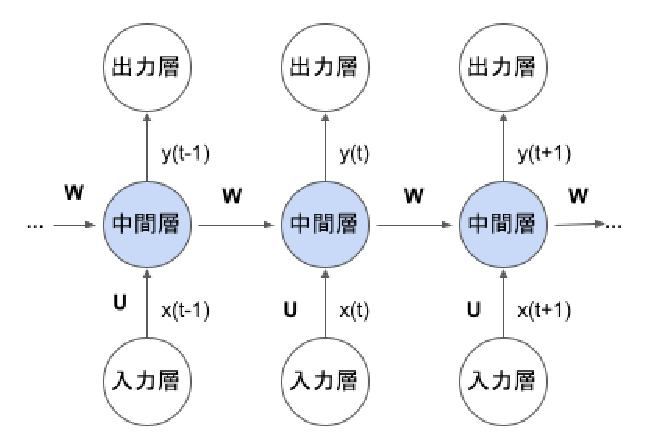
\includegraphics[width=\linewidth]{fig/chap2/RNN.eps}
  \caption{RNN モデル図}
  \label{fig:rnn}
\end{figure}



\vspace{-4mm}
\begin{equation}
    y(t) = f(U\bm{x}(t) + W\bm{s}(t - 1))
\end{equation}



入力 $x$ と $s(t - 1)$ により $s(t)$ が更新されていく.



\vspace{-4mm}
\begin{equation}
    y(t) = g(W\bm{s}(t))
\end{equation}












\subsection{LSTM}

LSTM(Long Short-Term Memory)は,RNN の欠点を補うようにして構築されたニューラルネットワークモデルである.
これは,1997 年に Sepp Hochreiter や J\"{u}rgen Schmidhuber が発表したモデルであり,時系列データを扱うことができる\cite{lstm}.
これは,長期記憶(Long Term Memory)と短期記憶(Short Term Memory)の二つを組み合わせて作られており,RNN では時刻が離れているデータ間の依存関係を学習することが難しかったという課題を克服するために開発されたモデルである.
近い過去を扱う短期記憶と遠い過去を扱う長期記憶が可能であるため,時系列データが長い場合には有効な場合が多い.
LSTM は RNN の中間層を LSTM block というメモリと入力ゲート及び忘却ゲート,出力ゲートの三つのゲートを持つブロックに置換することで実現されている.
メモリは入力の依存性を記憶している.
入力ゲートはメモリへ渡す入力を調整し,忘却ゲートはメモリの値を破棄する量を調整,出力ゲートはメモリの値を活性化関数に渡す量を調整する役割を持っている.



\vspace{-4mm}
\begin{equation}
    \bm{f}(t) = σ_g(U_f\bm{x}(t) + W_f\bm{h}(t - 1))
\end{equation}



\vspace{-4mm}
\begin{equation}
    \bm{i}(t) = σ_g(U_i\bm{x}(t) + W_i\bm{h}(t - 1))
\end{equation}



\vspace{-4mm}
\begin{equation}
    \bm{o}(t) = σ_g(U_o\bm{x}(t) + W_o\bm{h}(t - 1))
\end{equation}



\vspace{-4mm}
\begin{equation}
    \bm{c}(t) = \bm{f}(t)\odot \bm{c}(t - 1) + \bm{i}(t)\odot σ_c(U_c\bm{x}(t) + W_c\bm{h}(t - 1))
\end{equation} % 改行が都合よくできてない警告



\vspace{-8mm}
\begin{equation}
    y(t) = \bm{o}(t) \odot σ_h(\bm{c(t)})
\end{equation}



以上より,活性化関数 $σ$,入力層と中間層間の重み $U$,中間層と出力層間の重み $W$ を用いて忘却ゲート $\bm{f}(t)$ や入力ゲート $\bm{σ}(t)$,活性化ベクトル $\bm{o}(t)$,中間層の出力値 $\bm{h}(t)$,ネットワークの出力値 $y(t)$ を定義している.
$\odot$ はアダマール積を表しており,ベクトルの要素ごとに積を求める演算子である.




\begin{figure}[b]
  % \centering
  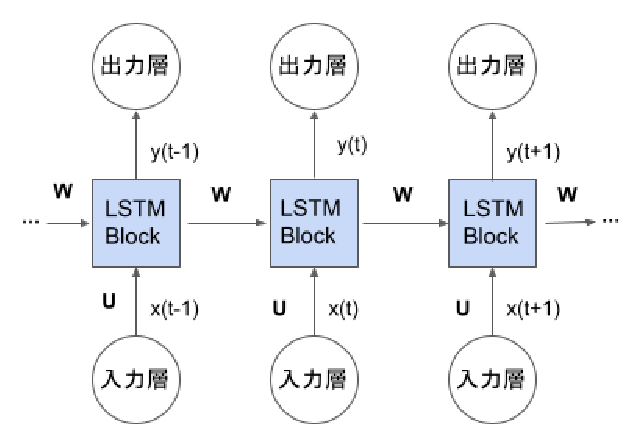
\includegraphics[width=\linewidth]{fig/chap2/LSTM.eps}
  \caption{LSTM モデル図}
  \label{fig:lstm}
\end{figure}
\vspace{7mm}











%3章 ニューラルネット
% \clearpage
% \newpage
\section{電力使用量予測実験}



\subsection{対象データ}

本研究では,東京電力パワーグリッド社が提供している電力使用量のデータを用い,2016 年 4 年から 2022 年 3 月までの期間を用いる.
時間ごとのデータは 24(時間)× 365(日)× 6(年)で 52560 個存在している.
日ごとのデータは 24 時間ごと,週ごとのデータは日ごとのデータを 7 日ごとにまとめて使用した.
電力使用量のデータの一部を図\ref{fig:denryoku}に示す.
2016 年 11 月 21 日から 2 週間分の電力使用量の波形を示している.
縦軸は電力使用量の $10^4$ kW,横軸は時間を表している.
図は,日ごとのデータを示しており,一日の間で規則的な波が現れている.
図より,日中は電力使用量が増え,夜間は減っていることが読み取れる.
本実験ではこのような電力使用量のデータを用いた.



\begin{figure}[b]
  % \centering
  % \hspace{-0.02\linewidth}
  \includegraphics[width=\linewidth]{fig/chap3/denryoku.eps}
  \caption{電力使用量の元データ}
  \label{fig:denryoku}
\end{figure}












\subsection{異常値検出}

電力使用量が,トレンドから外れるような急激な変化点を以降では異常値と呼ぶ.
異常値は,台風や豪雪などの,異常気象による影響により現れる傾向が高い.
そのような異常気象のときの電力使用量を予測することが大きな課題であるが,これまでの研究では精度の高い予測ができていない.
用いた電力使用量には,異常値が多く含まれており,そのような点についても高い予測精度を示すことが可能になれば,適切な電力調整や化石燃料調達に役立つ.
本実験では,実測データから異常値検出を行うが,実際の予測では,天気や降水量などの電力使用量に関わる他要因も含め,異常値が現れそうな位置を検出することを想定している.


時系列データの平滑化には,移動平均という手法が存在し,大きく分類すると単純移動平均と加重移動平均,指数移動平均の 3 種類に分類できる.
移動平均とは,金融分野の分析や気象の分析に用いられる手法のことである.


単純移動平均とは,SMA(Simple Moving Average)と呼ばれ,直近の $n$ 個のデータを平均をとり,単純な重み付けをすることなく,平滑化を行う手法のことである.
しかし,重み付けがないため,過去のデータの影響を受けてしまう.


加重移動平均とは,WMA(Weighted Moving Average)と呼ばれ,重みを一定量ずつ線形に減らすことで平滑化を行う手法のことである.
直近のデータの重みを $n$ として,その一つ前のデータの重みを $n-1$ とする.
このように重みを 0 まで小さくしていくことで古いデータの重みを減らし,古いデータの影響を小さくする手法である.


指数移動平均とは,EMA(Exponential Moving Average)と呼ばれ,加重移動平均では線形に減らした重みを指数関数的に減少させる手法のことである.
単純移動平均と比べて直近のデータに影響を受けやすいという特徴がある.


まず,指数移動平均による時系列データの平滑化を行った.
期間 14 日ごとのデータを用いて移動標準偏差(Moving Standard Deviation)を計算し,同様に 14 日ごとの指数移動平均を計算する.
指数移動平均の計算結果が移動標準偏差から 1 倍以上大きい値を異常値として扱った.
図\ref{fig:outlier}に異常値を検出した結果を示す.
青色が元の波形,橙色の波形が EMA,橙色の点が異常値を表している.
図から読み取れるように,トレンドから大きく外れているところが異常値となっている.
評価は全区間と異常値のみを集めた区間の 2 区間に分けて行う.
それぞれの区間について RMSE や分散の指標により評価を行う.





\begin{figure*}[b]
  % \centering
  \includegraphics[width=\linewidth,height=115mm]{fig/chap3/outlier_fig.eps}
  \vspace{-8mm}
  \caption{異常値検出結果}
  \label{fig:outlier}
\end{figure*}












\subsection{RNN による予測手法}

本研究では,RNN に入力として時間ごとや日ごと,週ごとの電力使用量のデータを与える.
このデータから時間ごと,日ごと,週ごとの電力使用量の予測を行った.
用いたデータを,Train data と Test data が 8:2 になるように分割し,入力データとした.
入力系列の長さは 12 とした.
そのため,時間ごとの予測なら 12 時間の電力使用量のデータを入力し,次の 1 時間の電力使用量を予測するような予測方法である.
同様に,日ごと,週ごとの予測も行う.
最適化アルゴリズムは Adam を用い,学習率の初期値は 0.001,損失関数として平均二乗誤差を用いた.
活性化関数は ReLU,バッチサイズは 64 とし,epoch 数は validation loss が 10 回以上改善しなくなるまで繰り返すこととした.
層数と中間層の素子数を変化させることで予測を行った.
層数は 1 層,2 層,3 層を変化させ,素子数は 100 個,200 個,300 個を変化させることによって予測精度を調べた.
RMSE と分散を用いることによって,予測した電力使用量の予測結果の評価を行った.
また,RMSE の式は以下で定義される.



\vspace{-4mm}
\begin{equation}
    RMSE = \sqrt{\frac{1}{n} \sum_{i=1}^{n}(y_i - \hat{y_i})^2}
\end{equation}



$n$ はデータ数,$y$ と $\hat{y}$ はそれぞれ入力値と予測値である.











\subsection{LSTM による予測手法}

RNN のときと同様に,LSTM に入力として時間ごとや日ごと,週ごとの電力使用量のデータを与えた.
このデータから時間ごと,日ごと,週ごとの電力使用量の予測を行った.
用いたデータを,Train data と Test data が 8:2 になるように分割し,入力データとした.
入力系列の長さは 12 とした.
そのため,時間ごとの予測なら 12 時間の電力使用量のデータを入力した.
同様に,日ごと,週ごとの予測も行う.
最適化アルゴリズムは Adam を用い,学習率の初期値は 0.001,損失関数として平均二乗誤差を用いた.
活性化関数は ReLU,バッチサイズは 64 とし,epoch 数は validation loss が 10 回以上改善しなくなるまで繰り返すこととした.
層数と中間層の素子数を変化させることで予測を行った.
層数は 1 層,2 層,3 層を変化させ,素子数は 100 個,200 個,300 個を変化させることによって予測精度を調べた.
RMSE と分散を用いることによって,予測した電力使用量の予測結果の評価を行った.

















% 4章 実験
% \clearpage
% \newpage
\subsection{結果}



電力使用量の元データ,学習データとテストデータに対する予測結果を一例として図\ref{fig:lstm_predict}に示す.
電力使用量の元データは緑色,学習データの予測は青色,テストデータに対する予測は橙色で示している.






\begin{figure*}[b]
  % \centering
  \includegraphics[width=\linewidth]{fig/chap4/lstm_predict.eps}
  \caption{モデルの予測}
  \label{fig:lstm_predict}
\end{figure*}






RNN と LSTM を用いて,時間ごと,日ごと,週ごとの電力使用量を予測した結果を表\ref{tab:rnn-time}に示す.
これは,RMSE と分散を用いて,Test data について予測結果を評価した表である.





\begin{table}[t]
\centering
  \caption{RNN を用いた時間ごとの予測}
  \vspace{3mm}
  \begin{tabular}{|l||c|}  \hline
    RMSE / 分散 & Test(全区間) \\ \hline \hline
    1 層(75)  & 0.0177 / 0.0323 \\ \hline
    1 層(100) & 0.0168 / 0.0349 \\ \hline
    1 層(125) & 0.0207 / 0.0319 \\ \hline

    2 層(100) & 0.0173 / 0.0338 \\ \hline
    2 層(125) & 0.0172 / 0.0329 \\ \hline
    2 層(150) & 0.0176 / 0.0338 \\ \hline

    3 層(100) & 0.0184 / 0.0320 \\ \hline
    3 層(125) & 0.0163 / 0.0334 \\ \hline
    3 層(150) & 0.0180 / 0.0338 \\ \hline
  \end{tabular}
  \label{tab:rnn-time}
\end{table}


RNN を用いた時間ごとの予測結果は,3 層,ニューロン数 125 個のときが最も精度の良い予測となっていた.
時間ごとのデータはデータ数が多く,層を重ねることで複雑な予測に対応しているためこの結果となっている.






\begin{table}[t]
\centering
  \caption{LSTM を用いた時間ごとの予測}
  \vspace{3mm}
  \begin{tabular}{|l||c|}  \hline
    RMSE / 分散 & Test(全区間) \\ \hline \hline
    1 層(75)  & 0.0158 / 0.0323 \\ \hline
    1 層(100) & 0.0148 / 0.0320 \\ \hline
    1 層(125) & 0.0176 / 0.0325 \\ \hline

    2 層(100) & 0.0172 / 0.0316 \\ \hline
    2 層(125) & 0.0134 / 0.0330 \\ \hline
    2 層(150) & 0.0165 / 0.0323 \\ \hline

    2 層(100) & 0.0163 / 0.0344 \\ \hline
    3 層(125) & 0.0139 / 0.0333 \\ \hline
    3 層(150) & 0.0148 / 0.0349 \\ \hline
  \end{tabular}
  \label{tab:lstm-time}
\end{table}


表\ref{tab:lstm-time}より,LSTM を用いた時間ごとの予測結果は,2 層,ニューロン数 125 個のときが最も精度の良い予測となっていた.
RNN のときと同様に,層を重ねて複雑な予測に対応しているためこの結果となっている.


また,時間ごとの異常値区間の予測精度を表\ref{tab:ijou-time}に示す.



\begin{table}[t]
\centering
  \caption{区間ごとの予測精度(時間)}
  \vspace{3mm}
  \begin{tabular}{|l||c|c|}  \hline
    RMSE/分散  & 異常値以外の区間 & 異常値区間 \\ \hline \hline
    RNN   &  0.0186 / 0.0321 & 0.0148 / 0.0377 \\ \hline
    LSTM  &  0.0148 / 0.0309 & 0.0133 / 0.0373 \\ \hline
  \end{tabular}
  \label{tab:ijou-time}
\end{table}



RMSE の結果は異常値区間の方が低くなっていることが読み取れる.
分散の値は大きくなっており,精度が高くないことがわかる.
RNN と LSTM では LSTM の方が区間別にみても精度が高くなっている.






\begin{table}[t]
\centering
  \caption{RNN を用いた日ごとの予測}
  \vspace{3mm}
  \begin{tabular}{|l||c|}  \hline
    RMSE / 分散 & Test(全区間) \\ \hline \hline
    1 層(100) & 0.095 / 0.044 \\ \hline
    1 層(125) & 0.091 / 0.041 \\ \hline
    1 層(150) & 0.093 / 0.042 \\ \hline

    2 層(100) & 0.094 / 0.042 \\ \hline
    2 層(125) & 0.093 / 0.041 \\ \hline
    2 層(150) & 0.098 / 0.041 \\ \hline

    3 層(100) & 0.107 / 0.042 \\ \hline
    3 層(125) & 0.098 / 0.042 \\ \hline
    3 層(150) & 0.099 / 0.041 \\ \hline
  \end{tabular}
  \label{tab:rnn-day}
\end{table}


表\ref{tab:rnn-day}より,RNN を用いた日ごとの予測結果は,1 層,ニューロン数 125 個のときが最も精度の良い予測となっていた.
時間ごとのデータと比べて,日ごとのデータはデータ数が少ないため,層数は 1 層が一番良くなっているが,1 層から 2 層までで精度に大きな差は生まれていない結果となった.





\begin{table}[t]
\centering
  \caption{LSTM を用いた日ごとの予測}
  \vspace{3mm}
  \begin{tabular}{|l||c|}  \hline
    RMSE / 分散 & Test(全区間) \\ \hline \hline
    1 層(100) & 0.103 / 0.042 \\ \hline
    1 層(125) & 0.098 / 0.040 \\ \hline
    1 層(150) & 0.111 / 0.042 \\ \hline

    2 層(100) & 0.128 / 0.042 \\ \hline
    2 層(125) & 0.097 / 0.043 \\ \hline
    2 層(150) & 0.109 / 0.043 \\ \hline

    3 層(100) & 0.112 / 0.042 \\ \hline
    3 層(125) & 0.109 / 0.044 \\ \hline
    3 層(150) & 0.130 / 0.038 \\ \hline
  \end{tabular}
  \label{tab:lstm-day}
\end{table}


表\ref{tab:lstm-day}より,LSTM を用いた日ごとの予測結果は,2 層,ニューロン数 125 個のときが最も精度の良い予測となっていた.
時間ごとの予測結果と同じ結果となった.
また,RNN と LSTM どちらの予測も,時間ごとの結果と比べて RMSE や分散の値が大きくなっていることがわかる.


また,日ごとの異常値区間の予測精度を表\ref{tab:ijou-day}に示す.



\begin{table}[t]
\centering
  \caption{区間ごとの予測精度(日)}
  \vspace{3mm}
  \begin{tabular}{|l||c|c|}  \hline
    RMSE/分散  & 異常値以外の区間 & 異常値区間 \\ \hline \hline
    RNN   &  0.088 / 0.041 & 0.109 / 0.051 \\ \hline
    LSTM  &  0.088 / 0.043 & 0.116 / 0.055 \\ \hline
  \end{tabular}
  \label{tab:ijou-day}
\end{table}



日ごとのデータの区間ごとの予測精度では,RNN と LSTM ともに異常値区間の RMSE が低くなっていた.
分散は,異常値区間が大きくなり,予測精度が高くないことがわかった.
全区間で高い精度を示したのは RNN だが,区間ごとに計算しても同じ結果になったと言える.







\begin{table}[t]
\centering
  \caption{RNN を用いた週ごとの予測}
  \vspace{3mm}
  \begin{tabular}{|l||c|}  \hline
    RMSE / 分散 & Test(全区間) \\ \hline \hline
    1 層(100) & 0.194 / 0.061 \\ \hline
    1 層(125) & 0.172 / 0.065 \\ \hline
    1 層(150) & 0.187 / 0.065 \\ \hline

    2 層(100) & 0.178 / 0.059 \\ \hline
    2 層(125) & 0.175 / 0.064 \\ \hline
    2 層(150) & 0.182 / 0.062 \\ \hline

    3 層(100) & 0.180 / 0.062 \\ \hline
    3 層(125) & 0.157 / 0.062 \\ \hline
    3 層(150) & 0.181 / 0.062 \\ \hline
  \end{tabular}
  \label{tab:rnn-week}
\end{table}


表\ref{tab:rnn-week}より,RNN を用いた週ごとの予測結果は,3 層,ニューロン数 125 個のときが最も精度の良い予測となっていた.
データ数が一番少ない週ごとのデータであるが,予測結果は 3 層,ニューロン数 125 個であった.
しかし,1 層から 3 層までの予測結果では大きな差はない結果となっていた.





\begin{table}[t]
\centering
  \caption{LSTM を用いた週ごとの予測}
  \vspace{3mm}
  \begin{tabular}{|l||c|}  \hline
    RMSE / 分散 & Test(全区間) \\ \hline \hline
    1 層(100) & 0.199 / 0.048 \\ \hline
    1 層(125) & 0.167 / 0.050 \\ \hline
    1 層(150) & 0.234 / 0.051 \\ \hline

    2 層(100) & 0.214 / 0.049 \\ \hline
    2 層(125) & 0.201 / 0.051 \\ \hline
    2 層(150) & 0.223 / 0.045 \\ \hline

    3 層(100) & 0.166 / 0.048 \\ \hline
    3 層(125) & 0.162 / 0.052 \\ \hline
    3 層(150) & 0.190 / 0.048 \\ \hline
  \end{tabular}
  \label{tab:lstm-week}
\end{table}


表\ref{tab:lstm-week}より,LSTM を用いた週ごとの予測結果は,3 層,ニューロン数 125 個のときが最も精度の良い予測となっていた.
1 層,2 層,3 層で結果を比べると 3 層のときの結果が 1 層,2 層に比べて精度が高くなっていた.


また,週ごとの異常値区間の予測精度を表\ref{tab:ijou-week}に示す.



\begin{table}[t]
\centering
  \caption{区間ごとの予測精度(週)}
  \vspace{3mm}
  \begin{tabular}{|l||c|c|}  \hline
    RMSE/分散  & 異常値以外の区間 & 異常値区間 \\ \hline \hline
    RNN   &  0.171/ 0.071 & 0.211 / 0.072 \\ \hline
    LSTM  &  0.179 / 0.059 & 0.223 / 0.058 \\ \hline
  \end{tabular}
  \label{tab:ijou-week}
\end{table}



週ごとのデータの区間ごとの予測精度は,RNN と LSTM ともに異常値区間の方が RMSE の値が大きくなり,予測精度が低くなっていた.
RNN では分散は,僅かに異常値区間の方が精度が低く,LSTM では僅かに異常値区間の方が精度が高いという結果であった.





時間ごと,日ごと,週ごとの電力の予測を RNN と LSTM を用いて行ってきたが,予測精度が高かったものは全てニューロン数が 125 個であることがわかった.
よって,電力使用量の予測にはどちらのモデルを用いるときでもニューロン数を 125 個に設定することで高い精度が得られる.







% 5章 考察
% \clearpage
% \newpage
\section{考察}


時間ごとの予測結果は RNN の場合では 3 層,ニューロン数 125 個のとき,LSTM では 2 層,ニューロン数が 125 個のときが最も精度の良い予測となっている.
RNN は膨大な期間のデータを記憶することには向いていないため,少ない層数では予測できなかったものだと考えられる.
LSTM では,RNN とは異なり,長期記憶が可能になっていることから,層数は 2 層で予測できている.
RNN より LSTM の方が全体的に RMSE,分散どちらの数値も小さくなっており,LSTM の方が予測精度が高くなっていた.
また,異常値については,分散が大きくなっているため,異常値区間の電力使用量の予測は精度が高くないことがわかった.





日ごとの予測結果は,RNN の場合は 1 層,ニューロン数 125 個のとき,LSTM では 2 層,ニューロン数 125 個のときが最も精度の高い予測となっている.
RNN のときは,時間ごとのデータよりもデータ数が少ないために層数が 1 層で高い精度の予測ができたと考えられる.
LSTM では 2 層のときが精度が高くなっているが,1 層の結果と値に大きな差はなく,層数は RNN と LSTM どちらの場合も複雑に重ねる必要がない.
それぞれの結果を比較すると,RNN の方が全体的に RMSE と分散が小さくなっており,精度が高いといえる.
異常値区間については予測精度が低くなっていた.
時間ごとのデータの予測と同様に,日ごとのデータの予測も異常値区間の予測精度が高くないことがわかった.





週ごとの予測結果は,RNN の場合は 3 層,ニューロン数 125 個のとき,LSTM では 3 層,ニューロン数 125 個のときが最も精度の高い予測となっている.
RNN,LSTM ともに層数が多くなっている.
週ごとのデータでは,1 時間の電力使用量のデータを 24 時間分合わせ,さらに 7 日分合わせて作成している.
天気や気温などが不規則なことに関連して,1 週間の電力使用量は複雑なデータとなっている可能性が高い.
データ数が少ないため層数は少なくても予測できるとは考えられるが,週ごとのデータが複雑なデータとなっていることにより層数は RNN と LSTM どちらも 3 層が予測精度が高くなったものだと考えられる.
異常値区間については,全区間に比べてかなり予測精度が悪くなっていることがわかった.
これもデータ数が少ないこと,データが複雑なことにより精度が下がったものだと考えられる.




データ量によって RNN と LSTM どちらのモデルを用いるか,層数の設定は変える必要があることがわかった.
ニューロン数については,125 個がほとんどの結果において高い精度を示していた.
しかし,異なるニューロン数の結果と比べて大きく精度が高くなっているとはいえない.
今後は,用いた電力使用量のデータ量より長期のデータを用いて実験を行い,これが適切なニューロン数であるか検討する必要がある.





結果より,データ量が非常に多くなるほど LSTM が予測に向いており,反対にデータ量の少ない場合は RNN の方が予測に向いている傾向があることがわかった.
用いるデータの量に合わせて適切なモデルとそのモデル構造を選択することで,より精度の高い電力使用量の予測の実現に繋がる.
また,異常値区間については,精度が低くなっていたため,電力使用量以外の他要因を用いる必要があると考えられる.
そうすることにより,天気や降水量など,電力使用量の変化に影響する他要因からも予測が行えるようになるため,集合型のマルチモーダル入力による学習を行う必要がある.
集合型のマルチモーダル学習とは,電力使用量のみから電力使用量の予測を行うモデルと,天気から電力使用量の予測を行うモデルや降水量から電力使用量の予測を行うモデルをそれぞれ作り,それらの予測結果の多数決をとる手法である.
ここでいう予測結果は,前の時刻から次の時刻にかけての電力使用量の変化量を予測することを表す.
このように予測することで急激に電力使用量が変化する時刻を予測できるようになると考えられる.











% 6章 おわりに
% \clearpage
% \newpage
\section{おわりに}


本研究では,発電所の稼働状態を調整することや適切な化石燃料の調達のための電力使用量の予測を行った.
予測結果は RMSE や分散を用いて精度を評価した.
RNN や LSTM を用いた予測では,時間ごと,日ごと,週ごとについてそれぞれ適切なモデルが存在し,電力使用量のトレンドを予測することができるようになった.
今後は全区間においてより精度の高い精度を追求していく.
また,異常値区間の予測精度については,全区間の予測精度に比べて低くなっていた.
異常値は,天気や降水量,気温などの要因から起こる可能性が高い.
今回の実験では,電力使用量のみの単入力で予測をしたため,異常値の予測には対応できていなかったと考えられる.


今後の課題は,電力使用量の単入力での予測精度の向上を図ることである.
また,電力使用量のみを入力データとして扱うのではなく,天気や降水量などの他要因もマルチモーダルな入力として扱う深層学習モデルを構築することである.
これにより,電力使用量のトレンドのみではなく,他要因により現れる異常値についても詳細な予測ができるようになる.








% \onecolumn
% %参考文献リスト
% \clearpage
% \newpage


% \vspace{15mm}


% bibtex使ってねー♪
\bibliographystyle{unsrt}
\bibliography{sankou}


% %業績
% \clearpage
% \newpage
% \thispagestyle{myheadings}
% \markright{業績}
% \input{gyouseki.tex}








% 参考論文 5 個は出して,はじめにで,参照すること
% \begin{thebibliography}{99}%%You should change 1 to 10 when there are more than 9 references.
%
%%%%%%%%%%%%%%%%%%%%%%%%%%%%%%%%%%%%%%%%%%%%%%%
% \vspace{-5mm}
%%%%%%%%%%%%%%%%
% \bibitem{sankou1} 加藤恭義 光成友孝 築山洋,セルオートマトン法ー複雑系の自己組織化と超並列処理ー,森北出版,1998
% %%%%%%%%%%%%%%%%%%%%%
% \bibitem{sankou2}T.Tamura J.Kuroiwa S.Nara,Dynamical Pattern Sequences Generated by CA Rule Dynamics of Sound Data,SNSA'03, Shigetoshi, China,2003
% %%%%%%%%%%%%%%%%%%%%%%%%%
% \bibitem{sankou3}今井秀樹,情報理論,昭晃堂,2000
% %%%%%%%%%%%%%%%%%%%%%%%%
% \bibitem{sankou4}森下信,セルオートマトン 複雑系の事象化,養賢堂,(2003)
% %%%%%%%%%%%%%%%%%%%%%%%%%%%
% \bibitem{sankou5}合原一幸,カオス カオス理論の基礎と応用,サイエンス社,1997
% %%%%%%%%%%%%%%%%%%%%%%%%%%%%
% \bibitem{sankou6}L.Chua V.Sbtnev S.Yoon,A Nonlinear Dynamics Perspecive of Wolfram's New Kind of Science.PartⅢ:Predicting the Unpredictable,I.J.Bifurcation$\&$Chaos, vol.14, No.11, 3689-3820, 2004
%%%%%%%%%%%%%%%%%%%%%%%%%%%%%%%%%
%
% \end{thebibliography}
%
%%%%%%%%%%%%%%%%%%%%%%%%%%%%%%%%%%%%%%%

\end{document}
%%%%%%%%%%%%%%%%%%%%%%%%%%%%%%%%%%%%%%%%%%%%%%%%%%%%%%%%%%%%%%
